% Setup
\documentclass[a4 paper, 12pt]{article}

% Title
\title{HIGH FIDELITY}

% Margins
\usepackage{geometry}
\geometry{margin=2cm}

% Images
\usepackage{graphicx}
\usepackage{float}
\usepackage[export]{adjustbox}
\setlength{\intextsep}{5pt plus 2pt minus 2pt}
\setlength\belowcaptionskip{0ex}
\usepackage[font=footnotesize,skip=2pt]{caption}

% Paragraph
\setlength{\parindent}{0em}
\setlength{\parskip}{1em}

% Text Formatting
\usepackage[utf8]{inputenc}
\usepackage[english]{babel}

% List spacing
\usepackage{enumitem}
\setlist{noitemsep, topsep=0pt}
\setlist[enumerate]{parsep=5pt} 

% Text Color
\usepackage{xcolor}

% Hyperlinks
\usepackage{hyperref}
\hypersetup{
    colorlinks=true,
    linkcolor=black,
    filecolor=black,      
    urlcolor=blue,
}

% Appendix
\usepackage{appendix}

% Include pdf
\usepackage{standalone}
\usepackage{pdfpages}

% Borders
\usepackage{mdframed}

% Symbols
\usepackage{amssymb}

\usepackage{multicol}

\usepackage{tabulary}
\usepackage{array}
\newcolumntype{L}{>{\arraybackslash}m{4cm}}
\newcolumntype{V}{>{\arraybackslash}m{6cm}}



\definecolor{mygreen}{HTML}{008037}
\definecolor{myblue}{HTML}{004AAD}
\definecolor{myorange}{HTML}{FF914D}
%%%%%%%%%%%%%%%%%%%%%%%%%%%%%%%%%%%%%%%%%%
\begin{document}
    
\section{Iteration 3 - High Fidelity Prototype}
The high fidelity prototype builds on the medium fidelity prototype with appropriate design changes to reflect the analysis of the previous iterations, as well as additional functionality to provide a more realistic experience of the application. The interface and functionality of this prototype should be ready for the first release of \textit{foodie}.

    % 3.3.1 REVISED REQUIREMENTS
    \subsection{Revised Requirements/Conception Design}
    There are no changes to the informed models (personas or interaction scenarios). 

    \subsubsection{System Concept Statement}    
    The following metaphors will be applied/added to this next iteration.
        \begin{itemize}
            \item cross $\dashrightarrow$ rubbish bin - \textit{Update delete icon to be consistent with industry standard.}
            \item tuning $\dashrightarrow$ cog - \textit{The 'tune' metaphor did not match the users' mental models for setting default preferences. Tune metaphor remains for filtering.}
            \item house - \textit{User's considered the filter page the main page and consistently wanted to return here. Participant 2: "looking for home button in the top bar to go back" [20])}
            \item floppy disk - \textit{Need a familiar metaphor for added 'saving' functionality}
            \item replay - \textit{Industry standard for undo action.}
            \item rubbish bin with three lines - \textit{To remove all functionality on edit pages.}
        \end{itemize}

        \begin{figure} [H]
            \centering
            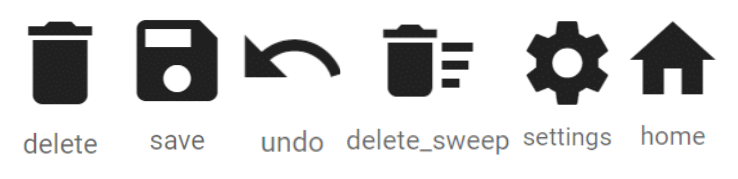
\includegraphics[width=0.3\textwidth, frame]
                {./High_Fidelity/High_Report/images/high_icons.PNG}  
                %{./images/high_icons.PNG}
            \caption{High Prototype Metaphors (Material Design) [59]}
        \end{figure}  

    \subsubsection{Design Principles}

    A couple of the design principles that were not being met in the previous iteration are being handled according to users. 
    \begin{itemize}
        \item Encourage collaboration - Users had no issues this iteration with viewing recommendations, recommending a visited place and sharing the compare list.
        \item Be familiar - There was no gap in mental models of any of the metaphors in this iteration.    
    \end{itemize}
       
    However, the following design principles have still not been adhered to in a satisfactory manner, causing continued issues for users.
    \begin{itemize}
        \item Customisation opportunities - Users had difficulty finding how they could set default preferences. This will be made clearer this iteration by updating the metaphor to a cog and the name to 'default preferences'. Users also wanted to be able to use their saved list to search and so an overlay will be introduced with more actions [68].
        \item Immediate access to actions - While users now had more action options on the compare page they also expected this overlay on other lists (saved/history). A similar overlay of actions will be added on these profile subpages. Also users wanted to be able to go straight to a place from the restaurant page so an action bar will replace the main bottom bar as it was not used. This position at the bottom of the screen ensures the easiest and quickest access for the users on mobile, which also adheres to Fitts Law [4, 53].
        \item Fluid navigation - There were still too many steps between pages, particularly for users who wanted to be directed straight to a restaurant without using the compare feature. A directions and call action will be added to the new action bar on the restaurant page.
        \item Clear direction \& guidance - The 'add to compare' button and favourites button were still hidden for many users. Both of these actions will be included in the action bar. This means there will be four options in the restaurant action bar, which adheres to Hicks Law [54].
    \end{itemize}
    
    Two new design principles will be introduced to assist with resolving issues identified in the medium fidelity prototype.
        \begin{itemize}            
            \item Purposeful movement - Users noted that were a number of times where they had to navigate through various pages to complete a simple task. For example, to go to a restaurant users need to arbitrarily choose a place on the map, add this restaurant to the compare list, select the compare tab, choose the restaurant from this list then select directions/call. To assist with meeting this design guideline an overview of restaurants using icons will be added to the maps as well as a bar on the action page to allow users to go straight to a restaurant.
            \item Consistency - The colours of icons was not consistent which caused confusion and errors from the users. For this iteration, a focus on consistency across the application will be applied, including both visual (colours) and functional (interactive elements) consistency [5]. To achieve this, dark pink fill will represent active states, fark pink outline will represent clickable buttons and the light pink fill will be when an action/button has been selected.
        \end{itemize}

    \subsubsection{System Requirements}
    As per the evaluations, it is evident that all system features are important to the range of users and all will be carried forward into this next iteration. However, for the requirement 'Track user history - Remember preferences and customise experience' this will be now split into three parts as the customisation of the application has more expectations from the user than originally anticipated.
        \begin{itemize}
            \item Track user history - Easily re-visit restaurants. \\
            \textit{This feature now specifically focuses on user's desire to be able to re-visit restaurants they have been too before as demonstrated by the interest in this feature during the medium evaluations. Additionally, the initial research states that while users eat out at least twice a week, they try new places sometimes leaving potentially have that time for places they love [24].}
            \item Remember preferences - Shortcuts for expert users. \\
            \textit{During the medium evaluations the ability to set preferences was not made obvious, despite user's enquiring if there was a feature to be able to save for later [10]}            
            \item Favourite restaurants - Alternative way to search for options. \\
            \textit{The capabilities of this feature are essential to Jessica and the clear definition provides expert users with more functionality. Also, in general users spend over 15 minutes searching through various options and don't want to repeat this process each time if avoidable [24].}
        \end{itemize}
   
    
    \subsubsection{UX Goals}  
    From the initial research and medium fidelity analysis, a number of the UX goals were not met adequately in the previous iteration.
        \begin{itemize}
            \item I want to re-visit restaurants that I enjoyed: User's did not have access to view more information about places in their history. 
                \begin{itemize}
                    \item \textit{Participant 2 \& 3: "I expected to be able to filter by history, use this to search." [9, 10]}
                    %\item \textit{Initial Research: All responded they try new places 'sometimes' which leaves remainder of time for places been before. [24]}  
                \end{itemize}            
            \item I want to dine out in my budget: The option to filter by budget was hidden and user's could not find it without assistance.
                \begin{itemize}
                    \item \textit{Participant 1 \& 2: "Want to be able to filter by price here but cant see that option, was looking for it first" [19,20]}
                    %\item \textit{Initial Research: Cost is the 3rd most important factor. [24]}
                \end{itemize}            
            \item I want to decide where to dine out in less than 20 minutes: There is no information about a restaurant before selecting on a map increasing the time to decide. 
                \begin{itemize}
                    \item \textit{Participant 4: "Looking for what is most popular, wondering for a way to see where I been before quickly [22]}
                \end{itemize}            
            \item I want to compare a variety of restaurants at once: The 'add to compare' button was hidden on the restaurant page, so users weren't aware this goal could be met or it was difficult to find. 
                \begin{itemize}
                    \item \textit{Participant 2 \& 5: "can't find the add to compare option" [20, 23]}
                \end{itemize}            
        \end{itemize}

    Also, from the medium prototype evaluations and interaction scenario analysis, there are three desires/expectations from users that did not match any of the existing UX goals. These goals will be added to the existing list to ensure usability for all users.
        \begin{itemize}
            \item I want to use my favourites to choose a restaurant.  
                \begin{itemize}
                    \item \textit{Participant 2 \& 3: "I expected to be able to filter saved, use this to search." [20,21]}
                    \item \textit{Jessica (scenario): Wants to be able to use her saved list as primary search feature}
                \end{itemize}
            \item I want to visit a place without comparing options. 
                \begin{itemize}
                    \item \textit{Participant 3: "want to go straight to a restaurant without adding to compare" [21]}
                    \item \textit{Matt (scenario): Wants to go to first best place.}
                \end{itemize}
            \item I want to save my preferences for next time. 
                \begin{itemize}
                    \item \textit{Participant 2: "not clear that can set defaults, but I would use this" [20]}
                    \item \textit{Sophie: Her diet doesn't change, setting preferences would save her time.}
                \end{itemize}          
        \end{itemize}


% 3.3.1 REVISED REQUIREMENTS
\subsection{High Fidelity Prototype}
Using the medium fidelity prototype as a strong foundation and the updated conceptual design, further steps to improve the usability, and therefore user experience, of the application were applied to a high fidelity prototype [57].

    \subsubsection{Interface Design}
    These were the main issues from the medium prototype and how they will be resolved:
    \begin{itemize}
        \item Filter by budget hidden $\dashrightarrow$ Add price to main filter page \\
        \textit{- David now has clear option to filter by what is most important to him}
        \item Difficulty setting default preferences $\dashrightarrow$ Replaced the icon with settings metaphor and added text, setting preferences is same as default filter page. \\
        \textit{- Sophie can now save her diet for next time}
        \item No overview on map  $\dashrightarrow$ Add classification icons to markers on interactive map            
        \item Can't go to restaurant without using compare feature $\dashrightarrow$ Add icon options to be able to get the information to go directly to a restaurant without adding to compare list. \\
        \textit{- Matt can now choose in less time as desired with just one option.}
        \item Expected to be able to filter saved/history lists $\dashrightarrow$ Added filter bar to these page similar to the map and menu pages. 
        \item Can't use saved list to access restaurant information $\dashrightarrow$ Added option to go to restaurant page from saved list using overlay.  \\
        \textit{- Jessica can now utilise her saved list better.}
    \end{itemize}

    This is an overview of the updated prototype, with the important aspect changes outlined and explained visually. 
    \begin{figure} [H]
        \centering
        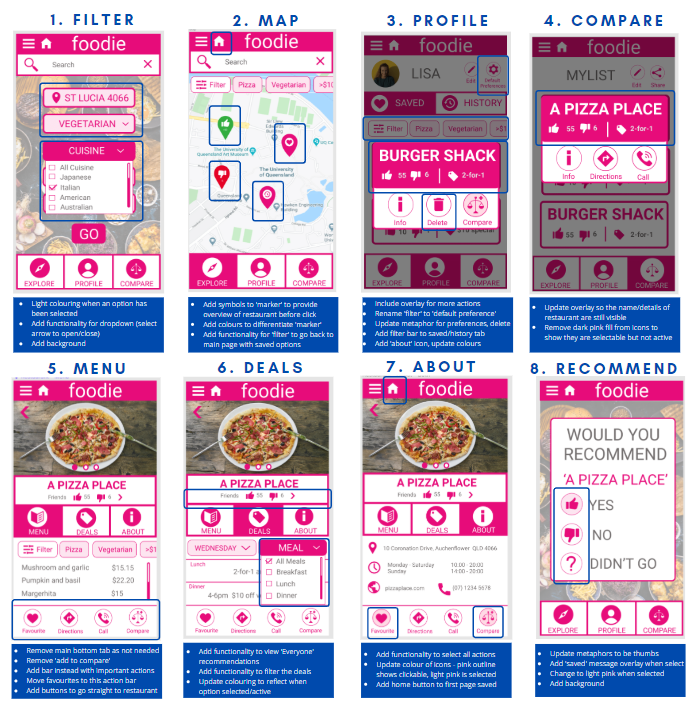
\includegraphics[width=\textwidth, frame]
            {./High_Fidelity/High_Report/images/high_proto_notes.PNG}  
            %{./images/high_proto_notes.PNG}
        \caption{High Prototype - Interface Modifications}
    \end{figure}  

    \subsubsection{Interface Functionality}
    Additional functionality has also been added to give the experts a more realistic experience of how the interface should behave.
    \begin{itemize}
        \item At least one option for each dropdown on main filter page.
        \item Basic preview of pages when adding default preferences.
        \item Change of state colour when adding a restaurant to compare or favourites.
        \item Preview of application status messages when saving a selection.
    \end{itemize}
    \begin{figure} [H]
        \centering
        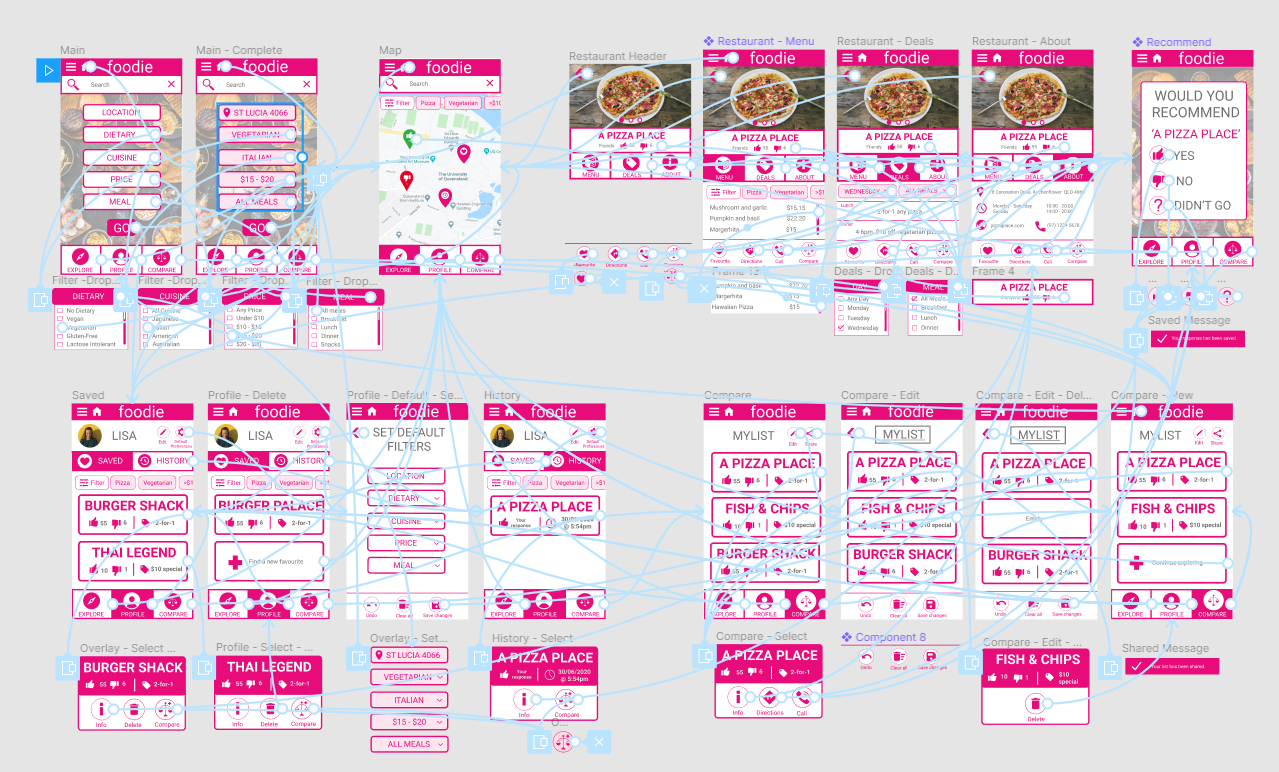
\includegraphics[width=\textwidth, frame]
            {./High_Fidelity/High_Report/images/high_proto_func.PNG}  
            %{./images/high_proto_notes.PNG}
        \caption{High Prototype - Interface Functionality}
    \end{figure} 



% High Fidelity Prototype Evaluation
\subsection{High Fidelity Prototype Evaluation}

    \subsubsection{Evaluation Methods}
    To effectively evaluate the high fidelity prototype, a heuristic evaluation was undertaken. This method requires HCI experts to critically assess the interface of the application against a set of criteria to determine whether it meets a minimum standard of usability [42]. This criteria will be a list of 10 heuristics which have been specifically selected for this application. By using experts there are fewer ethical and practical issues, and their knowledge can provide key insights into the general expectations of usability the domain and identify potential issues when all functionality is properly implemented. However, it is important to keep in mind that there is an increased possibility of trivial issues being identified and some larger issues overlooked as they are not evaluating through the eyes of the user [43].    

    There are two preparation steps before starting the heuristic evaluation [34]. The first is to determine the features of the application. These have been outline and updated continuously in the system requirements sections of the reports. The second step is the choose the set of heuristics with these features in mind. By looking at the \textcolor{mygreen}{SMART} [56], \textcolor{myblue}{Nielson's 10 general principles for interaction design} [44, 61, 70], and \textcolor{myorange}{HOMERUN} heuristics [48], 10 heuristics were chosen as criteria to determine their usability [43].
        \begin{enumerate}
            \item \textbf{\textcolor{mygreen}{Provide immediate notification of application status}}: 
            This is a refinement of \textit{\textcolor{myblue}{Visibility of system status}}, which states 'The system should always keep users informed about what is going on, through appropriate feedback within reasonable time' [44, 61, 70]. However, as this is a mobile application, the status must be immediate and due to screen size should be done non-intrusively where appropriate [43, 56].
            \item \textbf{\textcolor{mygreen}{Use a theme and consistent terms, as well as conventions and standards familiar to user}}: This is a combination of \textit{\textcolor{myblue}{Consistency and standards (use platform conventions)}} and \textit{\textcolor{myblue}{Match between system and the real world (for user)}}. Essentially, users should know exactly what words and actions mean, and these phrases should be familiar to the user with information appearing in a logical order [44, 61, 70]. Additionally, as this is a mobile application a theme should be used 'to ensure different screens look alike' and that the 'standards that users have come to expect in a mobile application' are used [43, 56].         
            \item \textbf{\textcolor{mygreen}{Prevent problems where possible; assist users should an error occur}}: This is a combination of \textit{\textcolor{myblue}{Help users recognize, diagnose and recover from errors}} and \textit{\textcolor{myblue}{Error prevention}}. Error message should be clear and concise with solution suggestions, and even better 'prevents a problem from occurring in the first place' [44, 61, 70]. It is essential that a mobile application 'is error-proofed as much as possible' [43, 56].        
            \item \textbf{\textcolor{myblue}{User control and freedom:}} 'Users often choose system functions by mistake and will need a clearly marked "emergency exit" to leave the unwanted state without having to go through an extended dialogue. Support undo and redo' [44, 61, 70].  
            \item \textbf{\textcolor{mygreen}{Each interface should focus on one task:}} Due to the  of mobile application, This heuristic is unique to mobile application as a result of their use cases (frequent interruptions) and screen space (less cluttering). This means 'only having the absolute necessary elements onscreen to complete that task' [43, 56].            
            \item \textbf{\textcolor{myblue}{Aesthetic and minimalist design:}} The original is \textit{\textcolor{myorange}{High quality content}} which is mainly for websites but highlights the important of providing functionality users want [48]. The mobile equivalent is \textit{\textcolor{mygreen}{A visually pleasing interface}} and focus on the forgiveness of users if the interface is attractive. The 'attractiveness' of an application is a qualitative measure with different opinions [43, 56]. Instead this heuristic focuses on the aesthetic of the app by assessing whether it is minimalist, which is the preferred design of today's mobile Users [47].       
            \item \textbf{\textcolor{myblue}{Recognition rather than recall:}} The HOMERUN equivalent is \textit{\textcolor{myorange}{Ease of use}} which states that 'users need to be able to find the information they need quickly and easily [48]. This is similar to \textit{\textcolor{mygreen}{Intuitive interfaces make for easier learning}}, which says similar for mobile interfaces in that they 'should be easy-to-learn whereby next steps are obvious' [43, 56]. Neither of these heuristics are clear about how the application should be achieving intuitiveness. Instead this heuristic focuses on minimises cognitive load by 'making objects, actions, and options visible' so that users dont need to remember each part of the process [44, 61, 70].
            \item \textbf{\textcolor{mygreen}{Design a clear navigable path to task completion:}} A more refined heuristic compared to \textit{\textcolor{myorange}{Relevant to users’ needs}} which measures whether the users are able to perform the task they want [48]. This heuristic measures whether users are 'able to see right away how they can interact with the application and navigate their way to task completion' [43, 56].     
            \item \textbf{\textcolor{mygreen}{Allow configuration options and shortcuts:}} A reworded revision of \textcolor{myblue}{Flexibility and efficiency of use}, it more appropriately identifies that the system should provide expert users with ability to tailor frequent actions [44, 61, 70]. 
            \item \textbf{\textcolor{mygreen}{Facilitate easier input:}} This heuristic is unique to mobile applications in that it focuses on making it easy to input content from the perspective of a mobile device [43,56]. 
        \end{enumerate}

    These were not chosen for this application:
        \begin{itemize}
            \item \textcolor{mygreen}{Display an overlay pointing out main features when appropriate or requested to help first-time users.:} This is similar to \textit{\textcolor{myblue}{Help and documentation}}, however there are no difficult elements of the application that need explaining and so no documentation is included for its use to be assessed by an expert [44, 61, 70].
            \item \textcolor{mygreen}{Use camera, microphone and sensors to lessen user’s  workload:} The only sensors used in this application is GPS which is adopted from other applications and so there is no unique factors to asses for this application. According to research and existing solution no other sensors would be appropriate [43, 56]. 
            \item \textcolor{mygreen}{Cater for diverse mobile environments (lighting, ambient noise, gloves, etc):} At this stage there have been no accommodations made for different use case environments and so there is nothing for users to assess against this heuristic [43, 56]. 
            \item \textcolor{myorange}{Often updated, Minimal download time, Unique to the online medium, Net-centric corporate culture supporting site:} None of these heuristics are relevant to the mobile application or available to be assessed at this stage of prototyping [48].            
        \end{itemize}

    The are three stages of a heuristic evaluation; briefing session, evaluation period and debriefing session. During the evaluation period, experts go through the features of the application individually twice [43]. The first time is to get a feel and understanding of the interface, and the second time through is to focus on the specific features and make notes [62]. During this second pass, according to chapter 13.4.2 of The UX Book, each expert 'individually browses through each part of the interaction design, asking the heuristic questions about that part'. The expert takes note of where and how the heuristic has been violated, how this would cause usability issues for the user and the probable effect on the user. They also rate the severity of the usability issue choosing between two options for three factors; occurrence (common, rare), impact (low, high) and perseverance (very, not). The combination of these factors provide a severity rating (0 to 4), and the mean of at least three evaluators ratings is satisfactory to determine the seriousness of the usability issue [63]. The debriefing session is an extension that could be used to brainstorm ideas for solutions [62].
        \begin{figure} [H]
            \centering
            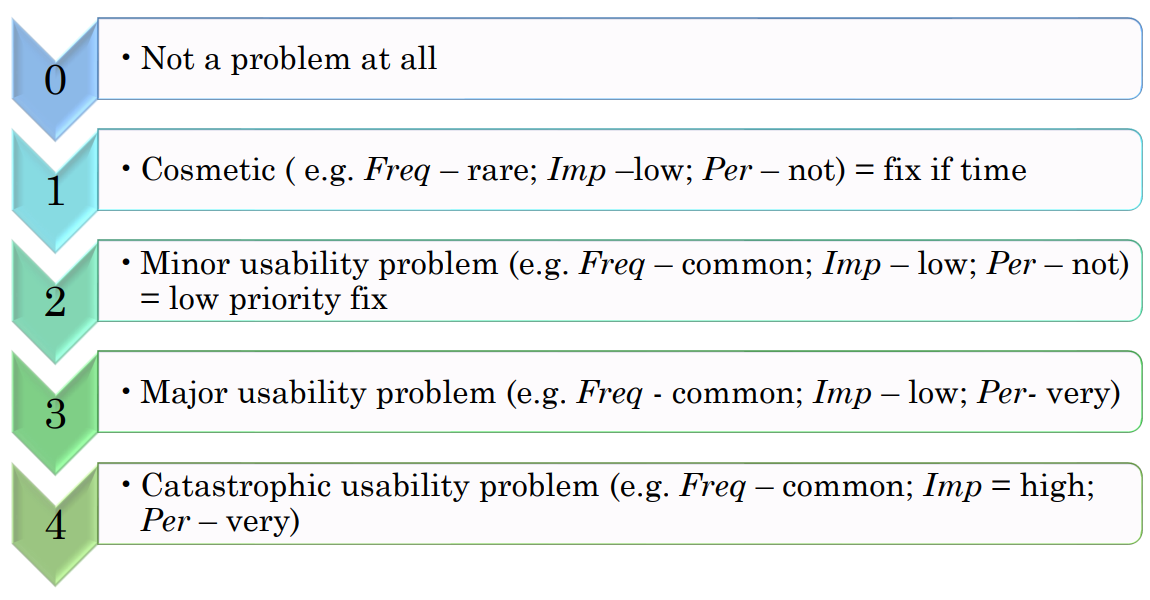
\includegraphics[width=0.6\textwidth, frame]
                {./High_Fidelity/High_Report/images/high_heuristic_severity.PNG}  
                %{./images/high_heuristic_severity.PNG}
            \caption{Heuristic Severity Ratings}
        \end{figure} 

    
    \subsubsection{Evaluation Protocol}
    The purpose of the protocol is the same as previous prototype evaluations. The protocol can be viewed in \hyperref[sec:B.1]{Appendix C.1}. To guide the experts through the three stages of the heuristic evaluation, after commencing the online call, the experts are provided with a link to a Google Forms. The form can be viewed in \hyperref[sec:C.2]{Appendix C.2}. The first step is the briefing session where the expert is given an overview of the task and expectations, and asked to complete a consent form. The second stage is completing the heuristic evaluation. The expert is given a list of 14 tasks, each of which pass through every page and feature of the application. The expert is asked to complete each task at their own speed with guidance when/if an error occurs.  They are provided with a link to the high fidelity prototype on figma. The slides can be viewed in \hyperref[sec:C.3]{Appendix C.3}.
        
    After the user has completed all of the tasks and expresses they feel confident with the system they are directed back to the Google Forms to prepare for the second pass. During the second pass of the application, the expert is again asked to complete each of the tasks however this time they are to specifically evaluate the usability of the system against the chosen heuristics. There are ten heuristics that were identified as part of the preparation for the evaluation. On the Google Forms, the experts are provided a link to a Google Sheets where there is a tab called HEURISTICS which lists and describes each of the heuristics. In the sheet is a second tab for the expert to fill out their notes with the appropriate headings, including the severity rating factors. The tabs of the sheet can be viewed \hyperref[sec:C.4]{Appendix C.4}. The expert uses the same link to the prototype to evaluate each task against these heuristics. After they are satisfied they have identified all the current issues the session ends.
    
    This evaluation included 5 experts as this would identify at least 75\% of the evaluations [43]. One of the evaluators also took part in the low fidelity evaluation and another has participated in all three evaluations. This range of familiarity with the application may provide the identification of some unique issues and ensures that all previous issue were addressed. Raw notes are in \hyperref[sec:C.5]{Appendix C.5}. 

    \subsubsection{Evaluation Results}
    From the heuristic evaluation there were a range of issues identified. Where more than one evaluator has noted the issue the mean of the severity factor responses has been taken. Also in this case, the heuristic that was consistent amongst all answers was chosen or a judgment call was made for the most appropriate. \\
    \begin{tabular}{|V|l|l|l|l|}
        \hline
        \textbf{Issue} & \textbf{\#Experts} & \textbf{Heuristic} & \textbf{Factors} & \textbf{Severity} \\
        \hline \hline 
        \multicolumn{5}{|c|}{DROPDOWN} \\
            \hline \hline
            want to select whole box not just arrow & 4 & 10 & common,low,very & major \\    
            \hline
            want to select text not just box & 3 & 10 & common,low,very   & major \\
            \hline
            want to select anywhere to save option & 3 & 3, 8 & common,low,very  & major \\
            \hline \hline              
        \multicolumn{5}{|c|}{SAVED MESSAGE} \\
            \hline \hline
            save doesn't take user away from edit screen & 1 & 8 & common,low,very & major \\            
            \hline
            saved message has to be clicked out of and then back & 1 & 8, 4 & common,low,very & major \\
            \hline \hline
        \multicolumn{5}{|c|}{MAIN} \\
            \hline \hline
            reset option & 2 & 3 & rare,low,very & cosmetic \\
            \hline
            not clear what home icon refers to & 2 & 3 & rare,low,very & Cosmetic \\
            \hline \hline
        \multicolumn{5}{|c|}{COMPARE} \\
            \hline \hline
            too many steps to delete, edit page redundant & 4 & 8,3 & common,low,very & major \\            
            \hline \hline
        \multicolumn{5}{|c|}{RESTAURANT} \\
            \hline \hline
            no shortcut to compare/favourite & 2 & 9 & rare,low,not & cosmetic \\
            \hline 
            want to see more detail about reviews & 2 & 2 & common,low,not & minor \\
            \hline
            menu text area is small, lots scrolling & 1 & 7 & common,low,not & minor\\                
            \hline \hline
        \multicolumn{5}{|c|}{PROFILE} \\
            \hline \hline    
            not clear need to save defaults & 2 & 1,6 & common,high,very & catastrophic \\
            \hline
            cant add to favourite from history & 2 & 9 & rare,low,very & cosmetic \\
            \hline
            cant undo delete for saved & 1 & 4 & rare,low,not & cosmetic \\
            \hline
            not able to delete/modify history & 1 & 4 & rare,low,not & cosmetic \\
            \hline    
    \end{tabular}    


    %\begin{itemize}
        % \item DROPDOWN (Main, Default, Deals)        
        %     \begin{itemize}
        %         \item \textcolor{myblue}{want to select whole box not just arrow} \textit{(4 experts - heuristic 10 - common,low,very)}
        %         \item \textcolor{myblue}{want to select text not just box} \textit{(3 experts - heuristic 10 - common,low,very)}                
        %         \item \textcolor{myblue}{want to select anywhere to save option} \textit{(3 experts - 4, 10, 3,8 - common,low,very)}
        %     \end{itemize}    
        % \item MAIN
        %     \begin{itemize}
        %         \item reset option - [2 experts - 3 - rare,low,very] - Cosmetic
        %         \item home icon shouldn't be on this page - [1 expert - 3 - rare,low,very] - Cosmetic
        %     \end{itemize}
        % \item COMPARE
        %     \begin{itemize}
        %         \item too many steps to delete, edit page redundant [4 experts  - 4,9, 7,8, 2, 3 - rare, low, very]  - Cosmetic
        %         \item save doesn't take user away from edit screen [1 expert - 8,10 - common,high,very] - Catastrophic
        %     \end{itemize}
        % \item RESTAURANT
        %     \begin{itemize}
        %         \item no shortcut to compare/favourite [2 experts - 9 - (rare,low,not)] - Cosmetic
        %         \item want to see more detail about reviews - [2 experts - 2 - common,low,not] - Minor 
        %     \end{itemize} 
        % \item RECOMMEND
        %     \begin{itemize}
        %         \item saved message has to be clicked out of and then back [2 experts - 8, 1,4 - common,low,very] - Major
        %     \end{itemize}
        % \item HISTORY
        %     \begin{itemize}
        %         \item not able to delete/modify - 4 (rare,low,not) - Cosmetic
        %         \item cant add to favourite - [2 experts - 9 - rare,low,very]
        %     \end{itemize}
        %     \item SAVED
        %         \begin{itemize}
        %             \item cant undo delete - 4 (common,low,not)
        %         \end{itemize}
        %     \item DEFAULT
        %         \begin{itemize}
        %             \item not clear need to save - 6 (common,high,very), 1 (rare,high,not)
        %         \end{itemize}
        %     \item MENU
        %         \begin{itemize}
        %             \item text area is small, lots scrolling - 7 (common,low,very)
        %         \end{itemize}
        % \end{itemize}


    % \begin{itemize}
        % \item DROPDOWN (Main, Default, Deals)
        %     \begin{itemize}
        %         \item want to select text not just box- 3,10 (common,low,very), 10 (common,low,very), 10 (common,low,very)
        %         \item want to select whole box not just arrow - 8,10 (common,high,very), 10 (common,low,very), 10 (common,low,very), 10 (rare/low/very)
        %         \item want to select anywhere to save option - 4 (rare,low,very), 10 (common,low,very), 3,8 (common,high,not)
        %     \end{itemize}
    %     \item MAIN
    %         \begin{itemize}
    %             \item reset option - 3 (rare,low,very), 3,4 (rare,low,very)
    %             \item home shouldn't be here - 3 (rare,low,very)
    %         \end{itemize}
    %     \item COMPARE
    %         \begin{itemize}
    %             \item too many steps to delete, edit page redundant - 4,9 (rare,low,very), 7,8	(rare,high,very), 2 (common,low,very), 3 (rare,high,very)
    %             \item save doesn't take user away from edit screen - 8,10 (common,high,very)
    %         \end{itemize}
    %     \item RESTAURANT
    %         \begin{itemize}
    %             \item no shortcut to compare/favourite - 9 (rare,high,very), 9 (rare,low,very)
    %             \item want to see more detail about reviews - 2,10 (common,high,not), 2 (common,high,not)
    %         \end{itemize} 
    %     \item HISTORY
    %         \begin{itemize}
    %             \item not able to delete/modify - 4 (rare,low,easy)
    %             \item cant add to favourite - 9 (rare,low,very), 9 (rare,high,not)
    %         \end{itemize}
    %     \item RECOMMEND
    %         \begin{itemize}
    %             \item saved message has to be clicked out of and then back - 8 (common,low,very), 1,4 (rare,low,easy)
    %         \end{itemize}
    %     \item SAVED
    %         \begin{itemize}
    %             \item cant undo delete - 4 (common,low,not)
    %         \end{itemize}
    %     \item DEFAULT
    %         \begin{itemize}
    %             \item not clear need to save - 6 (common,high,very), 1 (rare,high,not)
    %         \end{itemize}
    %     \item MENU
    %         \begin{itemize}
    %             \item text area is small, lots scrolling - 7 (common,low,very)
    %         \end{itemize}
    % \end{itemize}


    \subsubsection{Evaluation Analysis}
     All of the heuristic violation results identified are according to this sample of experts, so while approximately 75\% may have been collected there is potential that another set of the same evaluations with different experts could yield different results. Additionally, many of the issues identified were only identified by 1 or 2 experts which provides unreliable results. A further step that could be taken would be to recontact the experts with the entire list of issues and ask them to rate each one. This was not available at this time.  

     From the results there are four issues where their severity rating can be considered reliable (more than 3 experts), all of which have been identified as having a major market impact. The first two of these issues relate to the small area of selectability of the dropdown boxes and their content. These violate \textbf{heuristic 10} and do not align with Fitts law as larger buttons/selection area and proximity between selections is better for the user. The following two issues both violate \textbf{heuristic 3} and \textbf{heuristic 8} as they require unnecessary steps from the users and increase the chance of unresolved errors occurring. When selecting an option on a dropdown menu users have to be careful about how they choose to exit the overlay or their option will not be saved, and when deleted an option from the compare list users have to carefully complete at least four steps without warning if the sequence is not correct. These issues cause frustration and confusion for the user. All of these four issues will definitely need to be rectified in the next iteration due to their agreed consensus from experts as major issues and so are important to fix [63].

     The remaining issues were only identified by one or two experts and so the severity rating is not entirely reliable. Looking at those rated by at least two experts, there are four cosmetic issues, one minor, and one catastrophic. Reviewing these violations objectively, these issues will be considered for the next iteration with lower priority than the major issues identified previously. The first issue has been labelled as catastrophic in violation of \textbf{heuristic 1} and \textbf{heuristic 6}, which occurs on both the default preferences and edit compare list page. Experts noted that it was not clear that on these edit pages the changes needed to be saved as not only was there no response from the application when the pages weren't saved but this was not required for similar behaviour in other areas of the application. The minor issue violates \textbf{heuristic 2} and relates to the inability to view more information about reviews on the restaurant page when selecting the icons, despite this being an expected behaviour and functionality from other rating systems. The next two issues violate \textbf{heuristic 9}, firstly by not allowing users to add a visited restaurant to favourites easily and secondly by not providing accelerators to the favourite and compare list from the restaurant page for expert users [49]. The final two cosmetic issues relate to the violation of \textbf{heuristic 3} on the main page due to the absence of a reset button and the confusing presence of the home icon. 
          
     The final issues have only been identified by one expert and include two cosmetic, one minor, one major and one catastrophic. These will need further evaluation to determine their actual severity rating. At this time the two cosmetic issues violate \textbf{heuristic 4} and both relate to the profile page in that restaurants in the history cannot be delete/modified and there is no option to confirm or undo a deletion from the saved list. The minor issue is that the text of the menu is too small which may cause lots of scrolling and violates \textbf{heuristic 7}. The major and catastrophic issue are both identified by the same expert whom stated that the saved messages violate \textbf{heuristic 8}. The major issue is that when the saved message pop-up appears users must click outside of it and then the back arrow to go back, and the catastrophic issue is that after selecting saved the user isn't taken directly back to the previous screen. This is an example of the rating of one expert is unreliable as these appear to be less serious issues than presented given the impact of other issues. 

     Overall, the reliable major usability problems will be adjusted with high priority. This will resolve all of the violations of \textbf{heuristic 10}. For the unreliable issues from two experts the catastrophic issue will be given next priority followed by the minor problems. This will resolve all violations of \textbf{heuristic 1,2} and \textbf{6}. The cosmetic issues in this list will be handled if there is time, which will handle \textbf{heuristic 3 and 9}. The issues identified by only one expert will be rated further by at least one other expert to determine the actual violation of \textbf{heuristics 4,7} and \textbf{8} before deciding their priority. According to the results there is no violation of \textbf{heuristic 5}.

% \begin{itemize}
%     \item (1) Provide immediate notification of application status \& (6) Recognition rather than recall: Both violated once by the same issue which occurred on both the default preferences and edit compare list page. Experts noted that it was not clear that on these edit pages the changes needed to be saved as not only was there no response from the application when the pages weren't saved but this was not required for similar behaviour in other areas of the application.
%     \item (2) Use conventions and standards familiar to the user: Experts noted the inability to view more information about reviews on the restaurant page by selecting the icons. This is an expected behaviour and functionality from other rating systems. This is a minor issue so it is low priority.
%     \item (3) Prevent problems where possible; assist users should an error occur: The first relates to the absence of a reset option on the main page. The second issue was that the home icon is evident on the page despite this being the home page, potentially confusing users with what the icon then means. Also, users options are not saved unless they select arrow exactly.
%     \item (4) User control and freedom: This heuristic was violated on the profile page by 2 separate issues. The first is that once an option is deleted from the saved it cannot be undone if this was a mistake and the second is that the user is unable to delete/modify an option from their history if it is incorrect. 
%     \item (5) Each interface should focus on one task: This was the only heuristic that was not violated.    
%     \item (7) Aesthetic and minimalist design: This was violated on the menu page according to one expert who stated the text was too small which would be problematic if the menu was long due to extended scrolling.   
%     \item (8) Design a clear navigable path to task completion: This issue relates to the process of deleting an option from the compare list. Currently users must select 'edit', then select the option, then select 'delete' then save then back.  
%     \item (9) Allow configuration options and shortcuts: Firstly, experts noted that there was no way to get to the compare or favourites page after adding a restaurant without going back to the map. Secondly, a restaurant in the history list could not be added to favourites without searching for it again.  
%     \item (10) Facilitate easier input: The issues all relate to the selectability of the dropdown boxes and their content. Currently only selecting the arrow icon and the tick box exactly will open/select an option.     
%     \end{itemize}



\end{document}


